\subsectionFrame{Technical Preliminaries}

\begin{frame}{LTI System Model}
  \begin{columns}[T,onlytextwidth]
    \begin{column}{0.58\textwidth}
      Channel as Block Model\\
      \vspace{1em}
      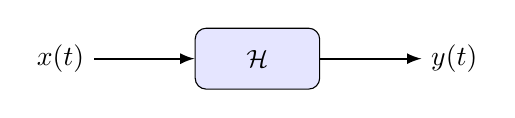
\begin{tikzpicture}[
    auto,
    >=latex,
    block/.style={draw, fill=blue!10, rounded corners, minimum height=2.2em, minimum width=4.5em, font=\small\bfseries},
    sum/.style={draw, fill=blue!10, circle, inner sep=0pt, minimum size=1.5em, font=\bfseries}
]
    \node (tx) at (0,0) {$x(t)$};
    \node[block] (lti) at (2.5,0) {$\mathcal{H}$};
    \node (rx) at (5.0,0) {$y(t)$};
    \draw[->, thick] (tx) -- (lti);
    \draw[->, thick] (lti) -- (rx);
\end{tikzpicture}
      \begin{itemize}
        \item System operator $\mathcal{H}$
        \item Transforms input signal $x(t)$ to output signal $y(t)$
      \end{itemize}
      \vfill
      System Operator under \ac{acro:lti} Properties\\
      \begin{itemize}
        \item \textbf{L}inear
          \begin{itemize}
            \item $\mathcal{H}\{\alpha x_1(t) + \beta x_2(t)\} = \alpha \mathcal{H}\{x_1(t)\} + \beta \mathcal{H}\{x_2(t)\}$
            \item Superposition principle
          \end{itemize}
        \item \textbf{T}ime \textbf{I}nvariant
          \begin{itemize}
            \item $\mathcal{H}\{x(t - \tau)\}=y(t-\tau)$
            \item Time delay $\tau$ of input equates to time delay $\tau$ of output
          \end{itemize}
      \end{itemize}
      \alert{Remark:} Real channels are inherently dynamic---covered in lecture 2 (coherence time)
    \end{column}
    %
    \begin{column}{0.38\textwidth}
      \begin{block}{Channel \ac{acro:cir}}
        Response to an ideal Dirac pulse $\delta(t)$\\
        \vspace{0.5em}
        \centering
        $h(t) = \mathcal{H}\{\delta(t)\}$
      \end{block}
      \begin{block}{\ac{acro:lti} Input-Output Relation}
        Convolution of input $x(t)$ with \ac{acro:cir} $h(t)$\\
        \vspace{0.5em}
        \centering
        $y(t) = x(t) * h(t)$ \\[0.2cm]
        $y(t) = \int_{-\infty}^{\infty} x(\tau) h(t - \tau) \,\mathrm{d}\tau$
      \end{block}
    \end{column}
  \end{columns}
\end{frame}

\begin{frame}{Fourier Transformation I}
  \begin{columns}[T,onlytextwidth]
    \begin{column}{0.58\textwidth}
      From Impulse Response to Transfer Function\\
      \begin{itemize}
        \item Time-domain \ac{acro:cir} $h(t)$ describes channel delay behavior
        \item \ac{acro:ft} maps \ac{acro:cir} to frequency domain \ac{acro:ctf}
        \item $h(t) \tf H(f)$
      \end{itemize}
      Basis Functions \& Eigenfunction Property\\
      \begin{itemize}
        \item Complex exponentials $\phi_f(t) = \ee^{\jj 2\pi f t}$ serve as orthogonal basis (kernel)
        \item Exponentials pass through unchanged except for complex scaling
        \item $\mathcal{H}\{\mathrm{e}^{\mathrm{j} 2\pi f t}\} = H(f) \cdot \mathrm{e}^{\mathrm{j} 2\pi f t}$
        \item Complex scalar $H(f)$ gives channel attenuation and phase rotation at frequency $f$
      \end{itemize}
    \end{column}

    \begin{column}{0.38\textwidth}
      \begin{block}{\ac{acro:ft} (Analysis)}
        Decomposition into spectrum\\
        \vspace{0.5em}
        \centering
        $H(f) = \int_{-\infty}^{\infty} h(t) \,\mathrm{e}^{-\mathrm{j} 2\pi f t} \,\mathrm{d}t$
      \end{block}

      \begin{block}{Inverse \ac{acro:ft} (\ac{acro:ift}) (Synthesis)}
        Reconstruction of time signal\\
        \vspace{0.5em}
        \centering
        $h(t) = \int_{-\infty}^{\infty} H(f) \,\mathrm{e}^{\mathrm{j} 2\pi f t} \,\mathrm{d}f$
      \end{block}
      \begin{block}{Orthonormality of Complex Exponentials}
        $$\left\langle \ee^{\jj 2 \pi f_1 t}, \ee^{\jj 2\pi f_2 t} \right\rangle = \delta(f_1 - f_2)$$
      \end{block}
    \end{column}
  \end{columns}
\end{frame}

\begin{frame}{Fourier Transformation II}
  \begin{columns}[T,onlytextwidth]
    \begin{column}{0.58\textwidth}
      Time-Frequency Uncertainty\\
      \begin{itemize}
        \item Direct consequence of the \ac{acro:ft} scaling property
        \item $x(at) \;\circ\!\!-\!\!\bullet\; \frac{1}{|a|} X\left(\frac{f}{a}\right)$
        \item Narrow time duration $\implies$ wide spectral occupancy
        \item Time-limited signals can never be strictly band-limited
      \end{itemize}
      \vspace{0.4em}

      Impact on Radio Standards\\
      \begin{itemize}
        \item Sharp transitions (e.g., rect pulse) cause slow $1/f$ spectral decay
        \item High sidelobes leak energy thereby causing interference
        \item Regulatory spectral masks strictly limit out-of-band emissions
      \end{itemize}

      \vspace{0.3em}
      \alert{Remark:} An optimal pulse must balance finite duration and low spectral sidelobes---covered in lecture 2 (root-raised-cosine)
    \end{column}

    \begin{column}{0.38\textwidth}
      \begin{block}{\ac{acro:ft} Example}
        \centering
        $\mathrm{rect}\!\left(\frac{t}{T}\right) \;\circ\!\!-\!\!\bullet\; T\,\mathrm{si}(\pi f T)$ \\[0.2cm]
        \footnotesize $\mathrm{si}(x) = \frac{\sin(x)}{x}$, zeros at $f = \pm \frac{k}{T}$

        \begin{figure}
          \centering
          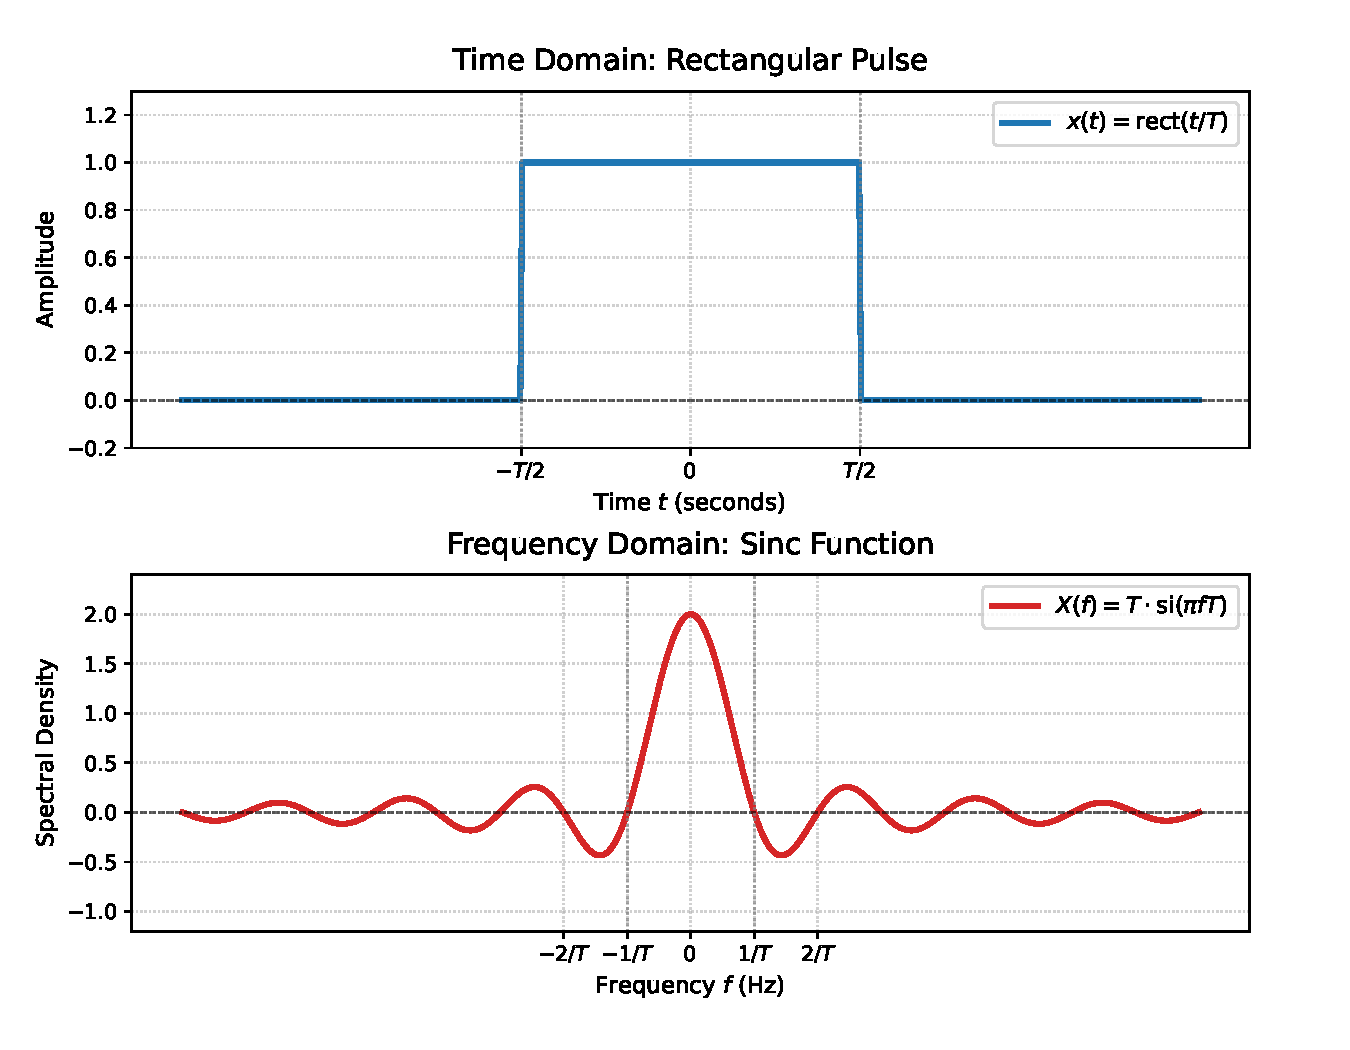
\includegraphics[width=1\linewidth]{images/section-1/rect_sinc.pdf}
          \caption{Rectangular Pulse and Si Function}
          \label{fig:placeholder}
        \end{figure}

      \end{block}
    \end{column}
  \end{columns}
\end{frame}

\begin{frame}{Fourier Transformation III}
  \centering
  Live demo: Frequency spectrum from the computer microphone
  \begin{itemize}
    \item scripts/section-1/live-spectrogram.py
  \end{itemize}
\end{frame}

\begin{frame}{Fourier Transformation IV}
  \label{1:FT4}
  \begin{columns}[T,onlytextwidth]
    \begin{column}{0.58\textwidth}
      Essential Fourier Properties\\
      \begin{itemize}
        \item Time Shifting (e.g. Propagation Delay)
          \begin{itemize}
            \item $x(t - \tau_0) \;\circ\!\!-\!\!\bullet\; X(f) \,\mathrm{e}^{-\mathrm{j} 2\pi f \tau_0}$
            \item Delay $\tau_0$ introduces a linear phase rotation across frequency
          \end{itemize}
        \item Frequency Shifting (e.g. Doppler Shift)
          \begin{itemize}
            \item $x(t) \,\mathrm{e}^{\mathrm{j} 2\pi f_\mathrm{D} t} \;\circ\!\!-\!\!\bullet\; X(f - f_\mathrm{D})$
            \item Doppler shift $f_D$ introduces linear phase rotation across time
          \end{itemize}
        \item Convolution Theorem
          \begin{itemize}
            \item $x(t) * h(t) \tf X(f) \cdot H(f)$
            \item Simplifies channel equalization from deconvolution to division
          \end{itemize}
        \item Sampling / Periodicity Duality
          \begin{itemize}
            \item Periodicity t/f $\Longleftrightarrow$ Sampling f/t
            \item \rlap{$\underbrace{x_\mathrm{s}(t) = x(t) \cdot \sum_{n=-\infty}^{\infty} \delta(t - n T_\mathrm{s})}_{\text{Sampling in Time}} \quad\circ\!\!-\!\!\bullet\quad \underbrace{X_\mathrm{s}(f) = \frac{1}{T_\mathrm{s}} \sum_{k=-\infty}^{\infty} X\!\left(f - \frac{k}{T_\mathrm{s}}\right)}_{\text{Periodification in Frequency}}$}
          \end{itemize}
      \end{itemize}
    \end{column}

    %\begin{column}{0.38\textwidth}
    %    \begin{block}{Hermitian Symmetry}
    %        For real physical signals $x(t) \in \mathbb{R}$:\\
    %        \vspace{0.4em}
    %        \centering
    %        $X(-f) = X^*(f)$ \\[0.2cm]
    %        \raggedright
    %        \footnotesize
    %        $\implies |X(-f)| = |X(f)|$ (even magnitude)\\
    %        $\implies \angle X(-f) = -\angle X(f)$ (odd phase)
    %    \end{block}
    %\end{column}
  \end{columns}
\end{frame}

\begin{frame}{Complex Baseband I}
  \begin{columns}[T,onlytextwidth]
    \begin{column}{0.58\textwidth}
      Why Complex Signals for Real Waves?\\
      \begin{itemize}
        \item Antennas emit and capture real-valued signals $s_\mathrm{BP}(t) \in \mathbb{R}$
        \item Communications signals usually narrowband ($B \ll f_\mathrm{c}$):
          \begin{itemize}
            \item Carrier $f_\mathrm{c}$ fixed in the GHz regime (e.g., $3.5\,\mathrm{GHz}$)
            \item Information encoded in amplitude $A(t)$ and phase $\phi(t)$
          \end{itemize}
        \item Simulating carrier oscillations at GHz rates is computationally expensive
      \end{itemize}
      \vspace{0.8em}
      Equivalent Complex \ac{acro:bb} Envelope\\
      \begin{itemize}
        \item Utilize complex numbers to combine amplitude and phase
        \item $s_\mathrm{BB}(t) = A(t) \,\mathrm{e}^{\mathrm{j} \phi(t)} \in \mathbb{C}$
        \item Describes signal independent of the carrier frequency
      \end{itemize}
    \end{column}

    \begin{column}{0.38\textwidth}
      \begin{block}{\ac{acro:bp} \ac{acro:bb} Transformation}
        \ac{acro:bp} as real projection of \ac{acro:bb} signal\\
        \vspace{0.5em}
        \centering
        $s_\mathrm{BP}(t) = \mathrm{Re}\Big\{ s_\mathrm{BB}(t) \,\mathrm{e}^{\mathrm{j} 2\pi f_\mathrm{c} t} \Big\}$
      \end{block}

      \begin{block}{Advantages}
        \begin{itemize}
          \item Spectrum centered around $0\,\mathrm{Hz}$
          \item Sample rate reduces from $2(f_\mathrm{c} + B/2)$ to $B$
          \item Clean mathematical framework for modulation and filtering
        \end{itemize}
      \end{block}
    \end{column}
  \end{columns}
\end{frame}

\begin{frame}{Complex Baseband II}
  \begin{columns}[T,onlytextwidth]
    \begin{column}{0.58\textwidth}
      Cartesian Decomposition of \ac{acro:bb}\\
      \begin{itemize}
        \item Split complex envelope into real and imaginary parts:
        \item $s_\mathrm{BB}(t) = I(t) + \mathrm{j} Q(t)$
        \item $I(t) = \mathrm{Re}\{s_\mathrm{BB}(t)\} = A(t)\cos\phi(t)$ (\textbf{In-Phase})
        \item $Q(t) = \mathrm{Im}\{s_\mathrm{BB}(t)\} = A(t)\sin\phi(t)$ (\textbf{Quadrature})
      \end{itemize}
      \vspace{0.8em}
      Orthogonal Carrier Modulation\\
      \begin{itemize}
        \item Expanding $s_{BP}(t)$ with Euler's identity
        \item $\mathrm{e}^{\mathrm{j} 2\pi f_\mathrm{c} t} = \cos \omega_\mathrm{c} t + \mathrm{j} \sin \omega_\mathrm{c} t$
        \item $s_\mathrm{BP}(t) = I(t)\cos(2\pi f_\mathrm{c} t) - Q(t)\sin(2\pi f_\mathrm{c} t)$
        \item Transmits two independent data streams over the same RF spectrum
      \end{itemize}
    \end{column}

    \begin{column}{0.38\textwidth}
      \begin{block}{\ac{acro:iq} Modulator Architecture}
        \centering
        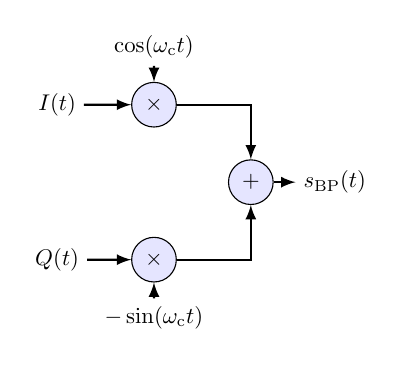
\begin{tikzpicture}[auto, >=latex, scale=0.82, every node/.style={scale=0.82}]
    \node (I) at (0,1.2) {$I(t)$};
    \node (Q) at (0,-1.2) {$Q(t)$};
    \node[draw,circle,fill=blue!10] (m1) at (1.5,1.2) {$\times$};
    \node[draw,circle,fill=blue!10] (m2) at (1.5,-1.2) {$\times$};
    \node (cos) at (1.5,2.1) {$\cos(\omega_\mathrm{c} t)$};
    \node (sin) at (1.5,-2.1) {$-\sin(\omega_\mathrm{c} t)$};
    \node[draw,circle,fill=blue!10] (sum) at (3.0,0) {$+$};
    \node (bp) at (4.3,0) {$s_\mathrm{BP}(t)$};
    \draw[->,thick] (I) -- (m1);
    \draw[->,thick] (Q) -- (m2);
    \draw[->,thick] (cos) -- (m1);
    \draw[->,thick] (sin) -- (m2);
    \draw[->,thick] (m1) -| (sum);
    \draw[->,thick] (m2) -| (sum);
    \draw[->,thick] (sum) -- (bp);
\end{tikzpicture}
      \end{block}
    \end{column}
  \end{columns}
\end{frame}

\begin{frame}{Why do we have Digital Communication Systems?}
  Disadvantages of Analog Systems
  \begin{itemize}
    \item Requires two physical signal traces for $I$ and $Q$
    \item Analog hardware impairments
  \end{itemize}
  Advantages of Digital Systems
  \begin{itemize}
    \item Complex numbers handled in memory/software
    \item Flexibility of the hardware platforms (Software-defined radio)
    \item Conditional access and encryption
    \item Error correction and information compression
    \item Storage of digital data
  \end{itemize}
\end{frame}

\begin{frame}{Discrete Fourier Transformation I}
  \begin{columns}[T,onlytextwidth]
    \begin{column}{0.5\textwidth}
      Discrete Counterpart of the \ac{acro:ft}\\
      \begin{itemize}
        \item The \ac{acro:dft} maps $N$ discrete time samples to $N$ discrete frequency bins
        \item \ac{acro:dft} kernel from \ac{acro:ft} kernel
        \item $\mathrm{e}^{-\mathrm{j} 2\pi f t} \quad\longrightarrow\quad \mathrm{e}^{-\mathrm{j} \frac{2\pi}{N} k n} = W_N^{k n}$
        \item Discrete complex exponentials $\phi_k[n] = \ee^{\jj \frac{2 \pi k n}{N}}$ serve as orthogonal basis
      \end{itemize}
      Intrinsic Periodicity of the \ac{acro:dft}
      \begin{itemize}
        \item Discrete harmonic basis is $N$-periodic
        \item $W_N^{(k + N)n} = W_N^{kn} \implies X[k + N] = X[k]$
        \item Time sequence implicitly treated as periodic
        \item $\tilde{x}[n] = x[n \bmod N]$
      \end{itemize}
    \end{column}

    \begin{column}{0.5\textwidth}
      \begin{block}{$N$-Point \ac{acro:dft} (Analysis)}
        Time sequence to discrete frequency\\
        \vspace{0.4em}
        \centering
        $X[k] = \sum_{n=0}^{N-1} x[n] \,\mathrm{e}^{-\mathrm{j} \frac{2\pi}{N} k n}$ \\[0.2cm]
        \footnotesize $k \in \{0, 1, \dots, N-1\}$
      \end{block}

      \begin{block}{$N$-Point \ac{acro:idft} (Synthesis)}
        Reconstruction of time samples\\
        \vspace{0.4em}
        \centering
        $x[n] = \frac{1}{N}\sum_{k=0}^{N-1} X[k] \,\mathrm{e}^{\mathrm{j} \frac{2\pi}{N} k n}$ \\[0.2cm]
        \footnotesize $n \in \{0, 1, \dots, N-1\}$
      \end{block}
      \begin{block}{Orthogonality of Discrete Complex Exponentials}
        $$\left\langle \ee^{\jj \frac{2 \pi k n}{N}}, \ee^{\jj \frac{2 \pi m n}{N}} \right\rangle= \begin{cases} N, & k = m \\ 0, & k \neq m \end{cases}$$
      \end{block}
    \end{column}
  \end{columns}
\end{frame}

\begin{frame}{Discrete Fourier Transformation II}
  \begin{columns}[T,onlytextwidth]
    \begin{column}{0.58\textwidth}
      \vspace{0.8em}
      \begin{itemize}
        \item Time Shifting
          \begin{itemize}
            \item Compare to \ac{acro:ft} (Slide \ref{1:FT4})
            \item $x\big[(n - n_0) \bmod N\big]= X[k] \, e^{-j \frac{2\pi}{N} k n_0}$
          \end{itemize}
        \item Frequency Shifting
          \begin{itemize}
            \item Compare to \ac{acro:ft} (Slide \ref{1:FT4})
            \item $X\big[(k - k_0) \bmod N\big] = x[n] \, e^{j \frac{2\pi}{N} k_0 n}$
          \end{itemize}
        \item Convolution Discrepancy Compared to \ac{acro:ft}
          \begin{itemize}
            \item Discrete \ac{acro:lti} channels perform linear convolution
            \item $y[n] = x[n] * h[n] = \sum_m h[m] x[n - m]$
            \item Multiplying two \ac{acro:dft}s yields circular convolution ($\circledast_N$)
            \item$x[n] \circledast_N h[n] \tf X[k] \cdot H[k]$ \\[0.2cm]
          \end{itemize}
      \end{itemize}
    \end{column}
    \begin{column}{0.38\textwidth}
      \begin{block}{Circular Convolution $\circledast_N$}
        \centering
        $x[n] \circledast_N h[n] = \sum_{m=0}^{N-1} h[m] \, x[(n - m) \bmod N]$
      \end{block}
    \end{column}
  \end{columns}
\end{frame}

\begin{frame}{Discrete Fourier Transformation III}
  \begin{columns}[T,onlytextwidth]
    \begin{column}{0.56\textwidth}
      \ac{acro:dft} is a linear transformation
      \begin{itemize}
        \item $N$-point \ac{acro:dft} acts as matrix-vector product:
          \begin{equation*}
            \mathbf{X} = \mathbf{F}_N \mathbf{x}
          \end{equation*}
        \item $\mathbf{x} = [x[0], \dots, x[N-1]]^T \in \mathbb{C}^N$
        \item $\mathbf{X} = [X[0], \dots, X[N-1]]^T \in \mathbb{C}^N$
        \item $\mathbf{F}_N$ is a symmetric matrix with entries $[\mathbf{F}_N]_{k,n} = W_N^{k \cdot n}$
      \end{itemize}
      \vspace{0.4em}
      Orthogonality \& \ac{acro:idft}
      \begin{itemize}
        \item Columns of $\mathbf{F}_N$ form an orthogonal basis:
          \begin{equation*}
            \mathbf{F}_N^H \mathbf{F}_N = N \mathbf{I}_N \implies \mathbf{F}_N^{-1} = \frac{1}{N}\mathbf{F}_N^H
          \end{equation*}
        \item \ac{acro:idft} matrix is conjugate transpose $\mathbf{F}_N^H$ scaled by~$1/N$
      \end{itemize}
      \vspace{0.4em}
    \end{column}

    \begin{column}{0.40\textwidth}
      \begin{block}{The \ac{acro:dft} Matrix $\mathbf{F}_N$}
        \centering
        \footnotesize
        $\mathbf{F}_N = \begin{bmatrix}
          1 & 1 & 1 & \dots & 1 \\
          1 & W_N^1 & W_N^2 & \dots & W_N^{N-1} \\
          1 & W_N^2 & W_N^4 & \dots & W_N^{2(N-1)} \\
          \vdots & \vdots & \vdots & \ddots & \vdots \\
          1 & W_N^{N-1} & W_N^{2(N-1)} & \dots & W_N^{(N-1)^2}
        \end{bmatrix}$
        \begin{itemize}
          \item With $W_N = \mathrm{e}^{-\mathrm{j}\frac{2\pi}{N}}$
        \end{itemize}
      \end{block}
    \end{column}
  \end{columns}
\end{frame}

\begin{frame}{Spatial Processing I}
  \begin{columns}[onlytextwidth]
    \begin{column}{0.48\textwidth}
      \begin{itemize}
        \item Plane wave = oscillation across distance and time
        \item Wave number $k_0$ = spatial phase velocity per meter ($\mathrm{rad/m}$)
        \item Wave vector $k$ = directional vector pointing along direction of propagation $\theta$
        \item Spatial sampling = antenna elements sample positions as \ac{acro:adc}s sample time
        \item Time--frequency duality maps to space--angle
      \end{itemize}
    \end{column}

    \begin{column}{0.48\textwidth}
      \begin{block}{Wave Basics}
        \begin{itemize}
          \item Wave propagation along time and frequency
          \item $s(\mathbf{r}, t) = \mathrm{e}^{\mathrm{j}(\omega t - \mathbf{k} \cdot \mathbf{r})}$
          \item Spatial frequency vector
          \item $k_0 = \frac{2 \pi}{\lambda}$
        \end{itemize}
      \end{block}

      \begin{block}{Time--Space Duality}
        \begin{tabular}{ll}
          \hline
          \textbf{Time Domain} & \textbf{Spatial Domain} \\
          \hline
          Time $t$ & Position $x$ \\
          Period $T_\mathrm{s}$ & Element Spacing $d$ \\
          Freq.\ $\omega$ & Wavenumber $k_0$ \\
          $f_\mathrm{s} \ge 2B$ & $d \le \lambda / 2$ \\
          \hline
        \end{tabular}
      \end{block}
    \end{column}
  \end{columns}
\end{frame}

\begin{frame}{Spatial Processing II}
  \begin{columns}[onlytextwidth]
    \begin{column}{0.48\textwidth}
      Uniform Linear Array (\ac{acro:ula})
      \begin{itemize}
        \item Plane wave arriving from angle $\theta$
        \item Wave travels extra $\Delta l$ per element
        \item Elements experience angle-dependent phase shift $\psi$ compared to reference element 0
        \item Array steering vector $\mathbf{a}(\theta)$
        \item $\mathbf{a}(\theta) = \begin{bmatrix} 1 & \mathrm{e}^{-\mathrm{j}\psi} & \dots & \mathrm{e}^{-\mathrm{j}(M-1)\psi} \end{bmatrix}^T$
          \item Spatial sampling without ambiguities if $d \le \frac{\lambda}{2} \iff |\psi| \le \pi$
      \end{itemize}
    \end{column}

    \begin{column}{0.50\textwidth}
      \centering
      \resizebox{\linewidth}{!}{\begin{tikzpicture}[
    >=Stealth,
    ray/.style={blue!75!black, thick, -{Stealth[length=2.2mm]}},
    wavefront/.style={cyan!80!black, thick}
]
    % Parameters
    \def\d{2.2}         % inter-element spacing
    \def\thetaAngle{30} % incidence angle from normal (deg)
    \def\rayLen{3.4}    % ray length

    % Array Elements (Sensors)
    \coordinate (S0) at (0, 0);
    \coordinate (S1) at (\d, 0);
    \coordinate (S2) at (2*\d, 0);

    % Baseline
    \draw[thick, gray!40] (-0.8, 0) -- (2*\d + 0.8, 0);

    % Broadside Normal at Element 0
    \draw[dashed, gray!70, thick] (0, 0) -- (0, 3.2);

    % Ray Origins (incoming from upper-left at angle theta from normal)
    \coordinate (R0) at ({-\rayLen*sin(\thetaAngle)}, {\rayLen*cos(\thetaAngle)});
    \coordinate (R1) at ({\d - \rayLen*sin(\thetaAngle)}, {\rayLen*cos(\thetaAngle)});
    \coordinate (R2) at ({2*\d - \rayLen*sin(\thetaAngle)}, {\rayLen*cos(\thetaAngle)});

    % Parallel Incoming Rays
    \draw[ray] (R0) -- (S0);
    \draw[ray] (R1) -- (S1);
    \draw[ray, blue!40, densely dashed] (R2) -- (S2);

    % Parallel Planar Wavefronts (orthogonal to ray)
    \foreach \offset in {1.4, 2.5} {
        \coordinate (W) at ({-\offset*sin(\thetaAngle)}, {\offset*cos(\thetaAngle)});
        \draw[wavefront] 
            ($(W) - 0.4*({cos(\thetaAngle)}, {sin(\thetaAngle)})$) -- 
            ($(W) + 2.8*({cos(\thetaAngle)}, {sin(\thetaAngle)})$);
    }
    \node[cyan!80!black, font=\scriptsize, rotate=\thetaAngle, above] 
        at ($({-2.5*sin(\thetaAngle)}, {2.5*cos(\thetaAngle)}) + 1.2*({cos(\thetaAngle)}, {sin(\thetaAngle)})$) 
        {Wavefront};

    % Exact projection P of S0 onto the ray entering S1:
    % P = S1 - (d*sin(theta)) * (sin(theta), -cos(theta))
    \coordinate (P) at ({\d - \d*sin(\thetaAngle)*sin(\thetaAngle)}, {\d*sin(\thetaAngle)*cos(\thetaAngle)});

    % Wavefront passing through S0 at the instant it hits Element 0
    \draw[teal!85!black, thick, dashed] 
        ($(S0) - 0.3*({cos(\thetaAngle)}, {sin(\thetaAngle)})$) -- 
        ($(P) + 0.5*({cos(\thetaAngle)}, {sin(\thetaAngle)})$);

    % Extra propagation path (Delta l) along ray to Element 1
    \draw[red!85!black, line width=1.6pt] (P) -- (S1) 
        node[midway, right=2pt, font=\footnotesize\bfseries, text=red!85!black] {$\Delta\ell$};

    % Exact Right-Angle square mark at P
    \coordinate (P_S0) at ($(P)!0.22cm!(S0)$);
    \coordinate (P_S1) at ($(P)!0.22cm!(S1)$);
    \coordinate (P_sq) at ($(P_S0) + (P_S1) - (P)$);
    \draw[gray!70, thick] (P_S0) -- (P_sq) -- (P_S1);

    % Angle theta arcs
    % 1. At Normal (Element 0)
    \draw[thick, red!85!black, ->] (0, 1.6) arc[start angle=90, end angle={90+\thetaAngle}, radius=1.6];
    \node[red!85!black, font=\footnotesize] at ({90 + \thetaAngle/2}:1.9) {$\theta$};

    % 2. Inside the geometric triangle at Element 0
    \draw[thick, red!85!black, ->] (0.7, 0) arc[start angle=0, end angle=\thetaAngle, radius=0.7];
    \node[red!85!black, font=\footnotesize] at ({\thetaAngle/2}:0.95) {$\theta$};

    % Sensor Antennas
    \foreach \i in {0, 1, 2} {
        \filldraw[fill=blue!10, draw=blue!85!black, thick] 
            (\i*\d - 0.16, -0.22) -- (\i*\d + 0.16, -0.22) -- (\i*\d, 0) -- cycle;
        \filldraw[blue!85!black] (\i*\d, 0) circle (1.8pt);
    }

    % Sensor Spacing dimension (d)
    \draw[{Stealth[length=1.4mm]}-{Stealth[length=1.4mm]}, thick] (0, -0.42) -- (\d, -0.42) 
        node[midway, fill=white, inner sep=1pt, font=\scriptsize] {$d$};

    % Sensor Labels (placed below spacing arrow to prevent overlap)
    \node[below, font=\scriptsize] at (0, -0.55) {Element $0$};
    \node[below, font=\scriptsize] at (\d, -0.55) {Element $1$};
    \node[below, font=\scriptsize] at (2*\d, -0.55) {Element $2$};
\end{tikzpicture}}

      \vspace{0.3em}
      \begin{beamercolorbox}[rounded=true,center,sep=3pt]{block body}
        \footnotesize
        \textbf{Path difference:} $\Delta \ell = d\sin\theta$ \\[2pt]
        \textbf{Phase shift:} $\psi = \frac{2\pi}{\lambda}\Delta \ell = \frac{2\pi d}{\lambda}\sin\theta$
      \end{beamercolorbox}
    \end{column}
  \end{columns}
\end{frame}

\begin{frame}{Spatial Processing III}
  \begin{columns}[onlytextwidth]
    \begin{column}{0.48\textwidth}
      Bartlett Beamformer
      \begin{itemize}
        \item Weight vector $\mathbf{w}(\theta)$ ``steers'' antenna array
        \item Maximizes output power for direction $\theta$ by selecting weights as
        \item $\mathbf{w}_\text{Bartlett}(\theta) = \frac{1}{M}\mathbf{a}(\theta)$
        \item Undo the phase shifts introduced by the channel
        \item Scan output power of the beamformer across $\theta$
        \item $P_{\mathrm{BF}}(\theta) = \mathbf{w}^H(\theta)\,\mathbf{R}_{xx}\,\mathbf{w}(\theta)$
      \end{itemize}
    \end{column}

    \begin{column}{0.48\textwidth}
      \begin{tikzpicture}[
    >=Stealth,
    thick,
    node distance=1.2cm,
    block/.style={draw=blue!85!black, fill=blue!10, rounded corners=2pt, minimum width=1.1cm, minimum height=0.6cm, font=\scriptsize, align=center},
    sum/.style={circle, draw=black, fill=gray!15, inner sep=0pt, minimum size=0.65cm, font=\normalsize}
]
    % Antenna Elements
    \foreach \m in {0, 1, 2} {
        \coordinate (ant\m) at (0, -\m*1.5);
        % Antenna triangle
        \filldraw[fill=blue!10, draw=blue!85!black] 
            ($(ant\m) + (-0.15, 0.15)$) -- ($(ant\m) + (0.15, 0.15)$) -- (ant\m) -- cycle;
        \filldraw[blue!85!black] (ant\m) circle (1.2pt);
        \draw (ant\m) -- ++(0.5, 0);

        % Weight multiplication block
        \node[block] (w\m) at ($(ant\m) + (1.4, 0)$) {$\times\, w_{\m}^*$};
        \draw[->] ($(ant\m) + (0.5, 0)$) -- (w\m) 
            node[midway, above, xshift=-4pt, font=\tiny] {$x_{\m}[n]$};
    }

    % Element labels
    \node[left, font=\tiny] at ($(ant0) + (-0.15, 0.05)$) {Element $0$};
    \node[left, font=\tiny] at ($(ant1) + (-0.15, 0.05)$) {Element $1$};
    \node[left, font=\tiny] at ($(ant2) + (-0.15, 0.05)$) {Element $M{-}1$};

    % Dots between Ant 1 and M-1
    \path (ant1) -- (ant2) node[midway, font=\scriptsize] {$\vdots$};
    \path (w1) -- (w2) node[midway, font=\scriptsize] {$\vdots$};

    % Summation Node
    \node[sum] (adder) at (3.1, -1.5) {$\Sigma$};

    % Connect weights to sum
    \draw[->] (w0.east) -| (adder.north);
    \draw[->] (w1.east) -- (adder.west);
    \draw[->] (w2.east) -| (adder.south);

    % Output y[n]
    \draw[->, very thick, blue!85!black] (adder.east) -- ++(1.1, 0) 
        node[right, font=\footnotesize, black] {$y[n]$};
\end{tikzpicture}
      \begin{block}{Output Signal Model}
        \begin{itemize}
          \item Snapshot vector: $\mathbf{x}[n] = \mathbf{a}(\theta_0)s[n] + \mathbf{n}[n]$
          \item Beamformer output: $y[n] = \mathbf{w}^H(\theta)\mathbf{x}[n]$
          \item Spatial covariance: $\mathbf{R}_{xx} = \mathbb{E}\{\mathbf{x}[n]\mathbf{x}^H[n]\}$
        \end{itemize}
      \end{block}
    \end{column}
  \end{columns}
\end{frame}

\begin{frame}{Spatial Processing IV}
  \centering
  Live demo: Bartlett beamformer visualization
  \begin{itemize}
    \item scripts/section-1/bartlett.py
    \item scripts/section-1/bartlett-multi-doa.py
  \end{itemize}
\end{frame}


\subsectionFrame{Standardization Preliminaries}

\begin{frame}{Radio Spectrum}
  \begin{columns}[T,onlytextwidth]
    \begin{column}{0.56\textwidth}
      What is the Radio Spectrum?
      \begin{itemize}
        \item Part of electromagnetic spectrum from $3\,\mathrm{Hz}$ to $3\,\mathrm{THz}$
        \item Finite natural resource used for wireless communication
        \item Backbone of modern telecommunication and broadcasting
      \end{itemize}
      \vspace{0.3em}
      Spectrum Allocation
      \begin{itemize}
        \item Globally coordinated by c{acro:itu}
        \item Divided into frequency bands assigned to specific services (TV, radio, mobile, satellite, radar, amateur)
      \end{itemize}
    \end{column}
    %
    \begin{column}{0.38\textwidth}
      \begin{block}{Frequency vs. Wavelength}
       \begin{itemize}
         \item Connection between frequency $f$ and wavelength $\lambda$
         \item $c = \lambda \cdot f$
         \item $c = \qty{299792458}{\meter\per\second}$ (in vacuum)
       \end{itemize}
      \end{block}
      \begin{alertblock}{Rules-of-Thumb}
        \begin{itemize}
          \item $\qty{1}{\giga\hertz} \rightarrow \qty{30}{\centi\meter}$
          \item $\qty{3}{\giga\hertz} \rightarrow \qty{10}{\centi\meter}$
          \item $\qty{10}{\giga\hertz} \rightarrow \qty{3}{\centi\meter}$
        \end{itemize}
      \end{alertblock}
    \end{column}
  \end{columns}
\end{frame}

\begin{frame}{Radio Spectrum by c{acro:itu}}
  \begin{figure}
    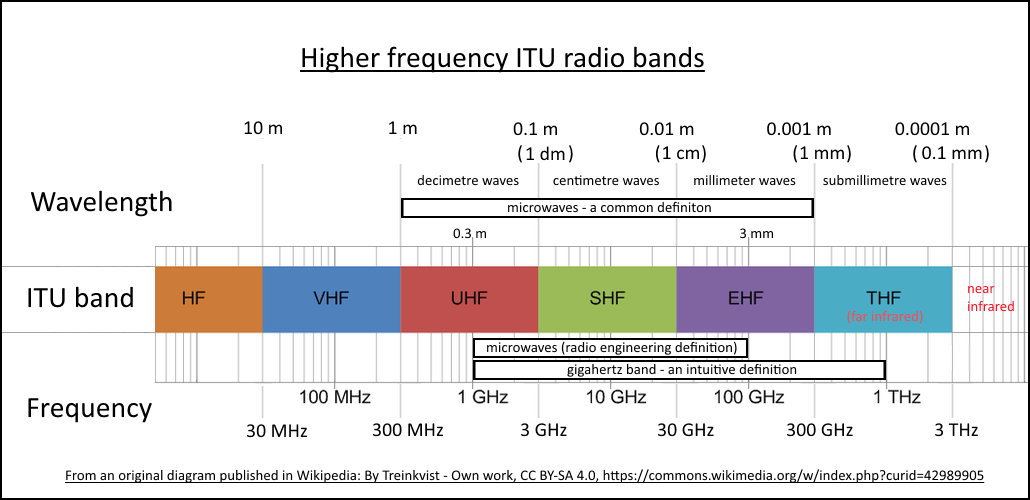
\includegraphics[width=1\linewidth]{images/section-1/radio-spectrum-itu.png}
    \caption{Radio Spectrum and c{acro:itu} Frequency Bands~\cite{radio-spectrum-itu}}
  \end{figure}
\end{frame}

\begin{frame}{Radio Spectrum Allocation USA}
  \begin{figure}
    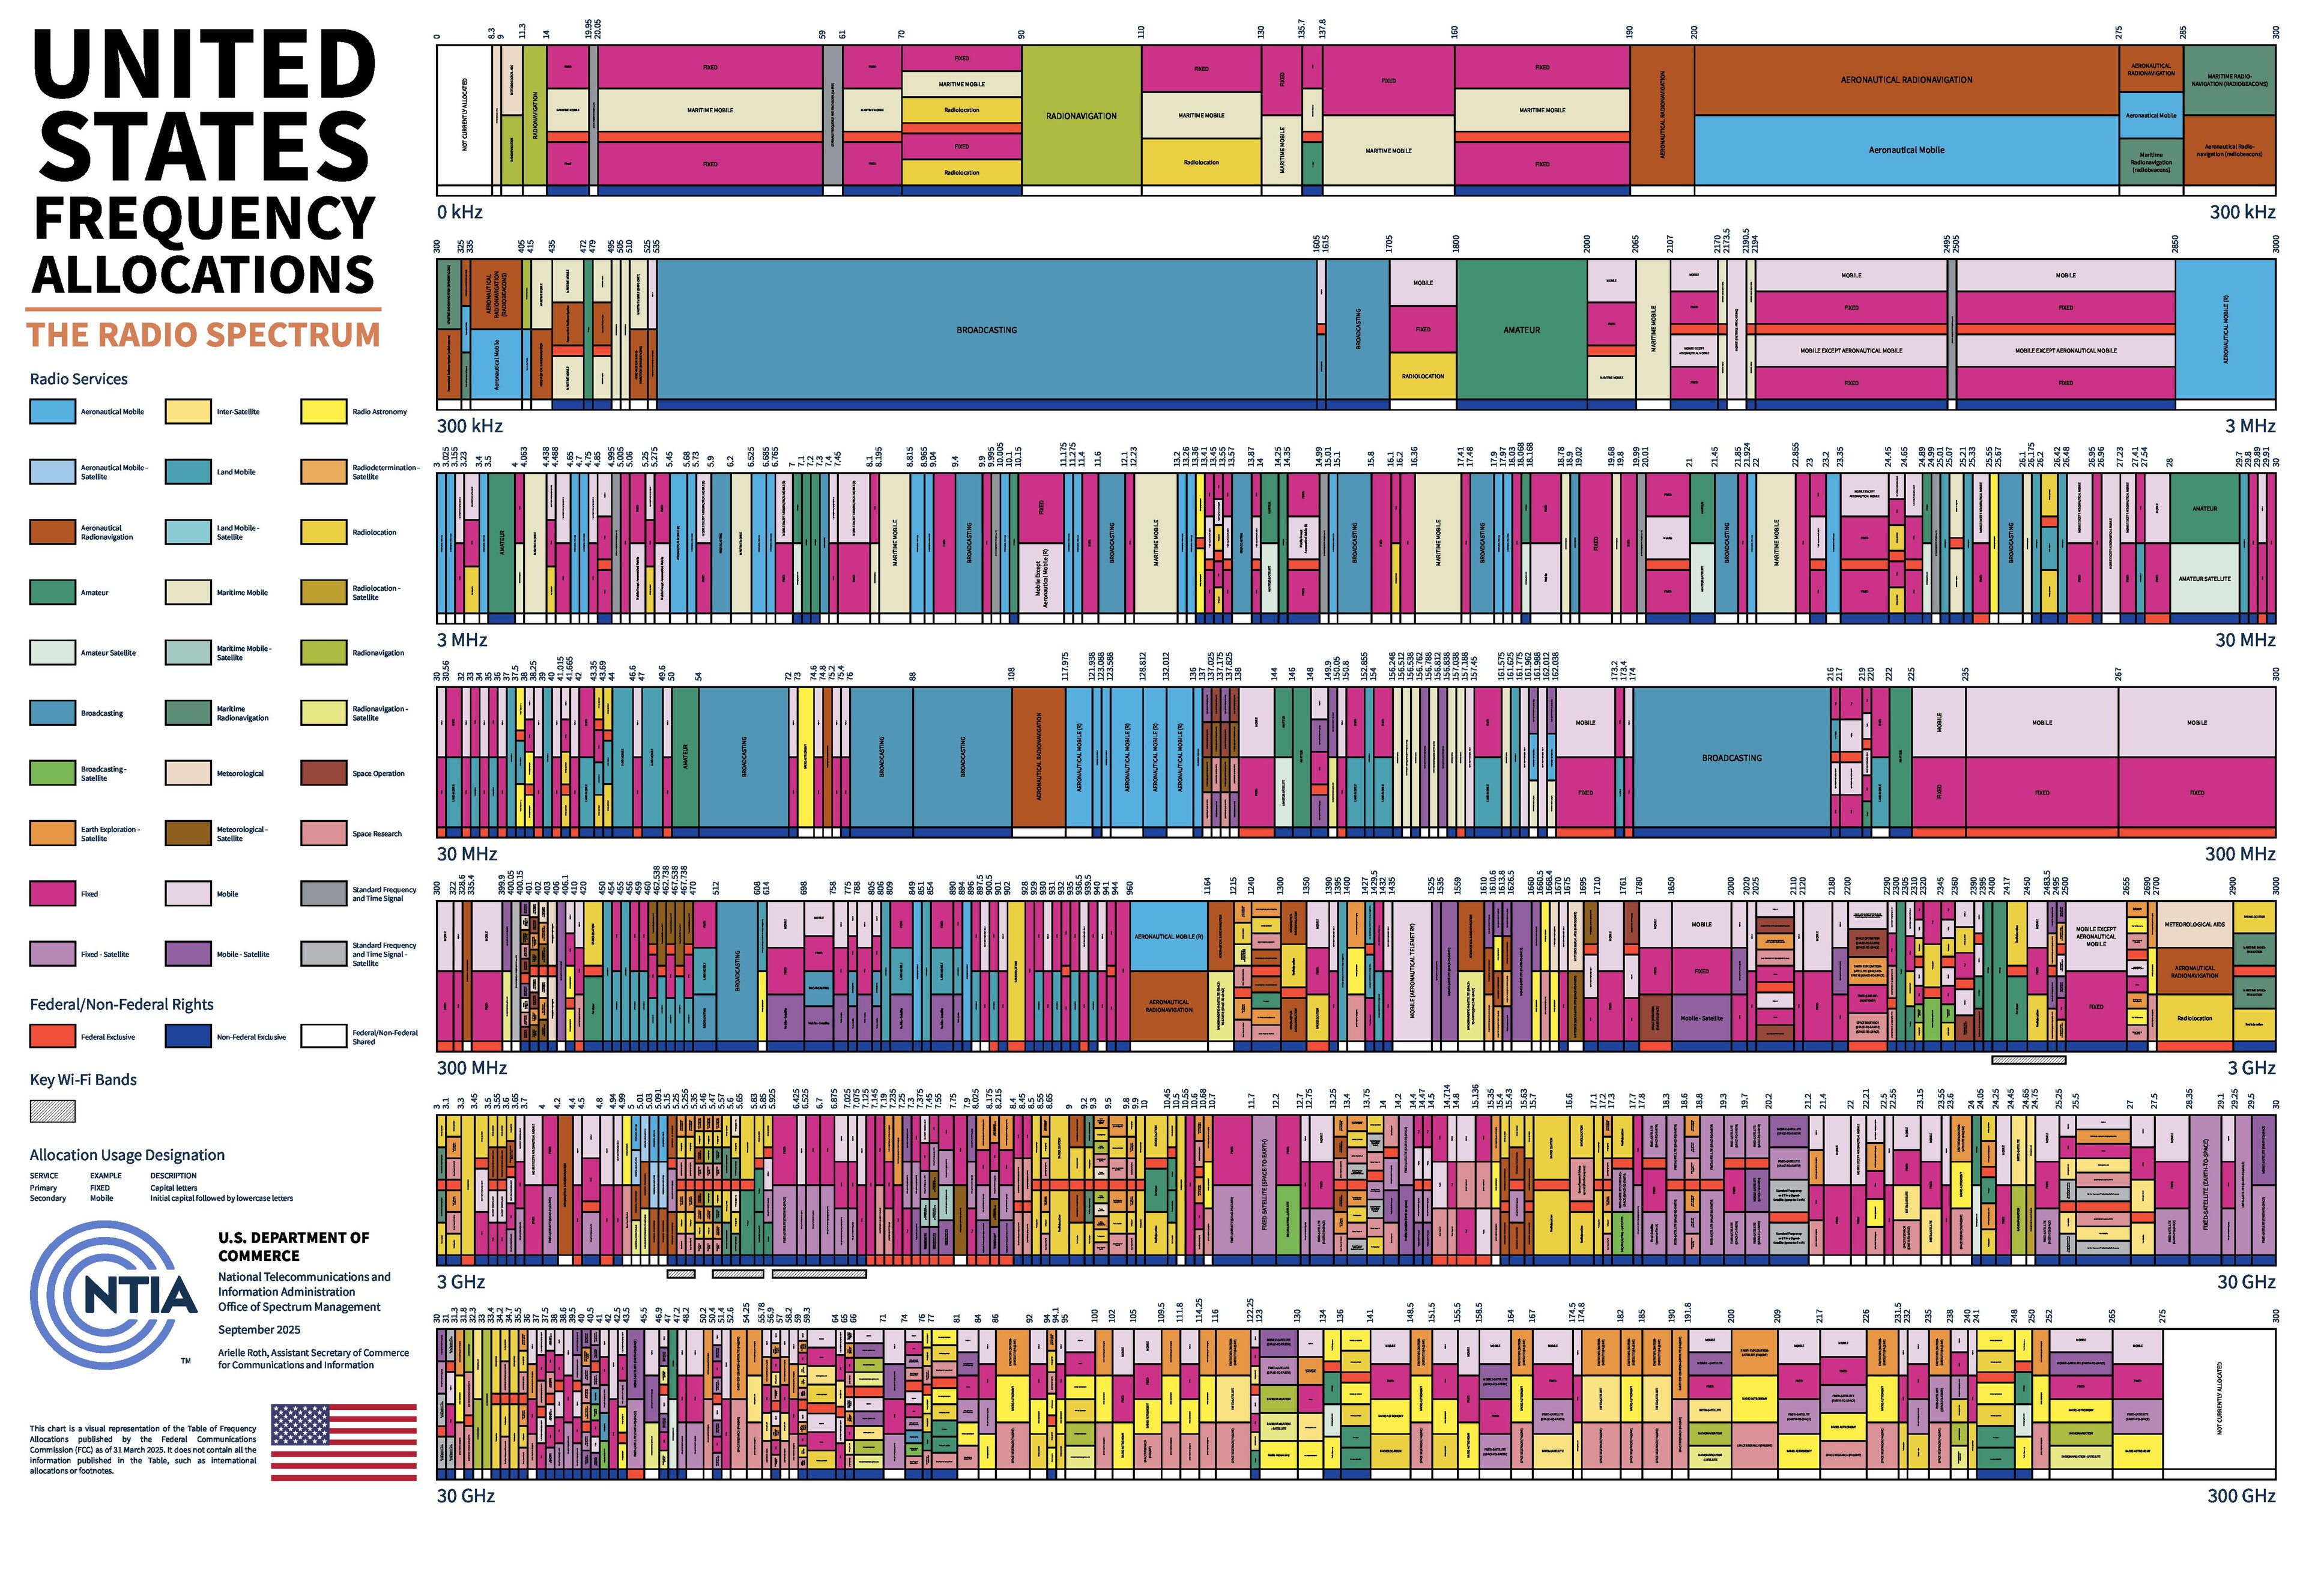
\includegraphics[width=0.7\linewidth]{images/section-1/radio-spectrum-usa.jpg}
    \caption{Radio Spectrum Allocation USA~\cite{radio-spectrum-usa}}
  \end{figure}
\end{frame}

\begin{frame}{Allocation Example I}
  \begin{figure}
    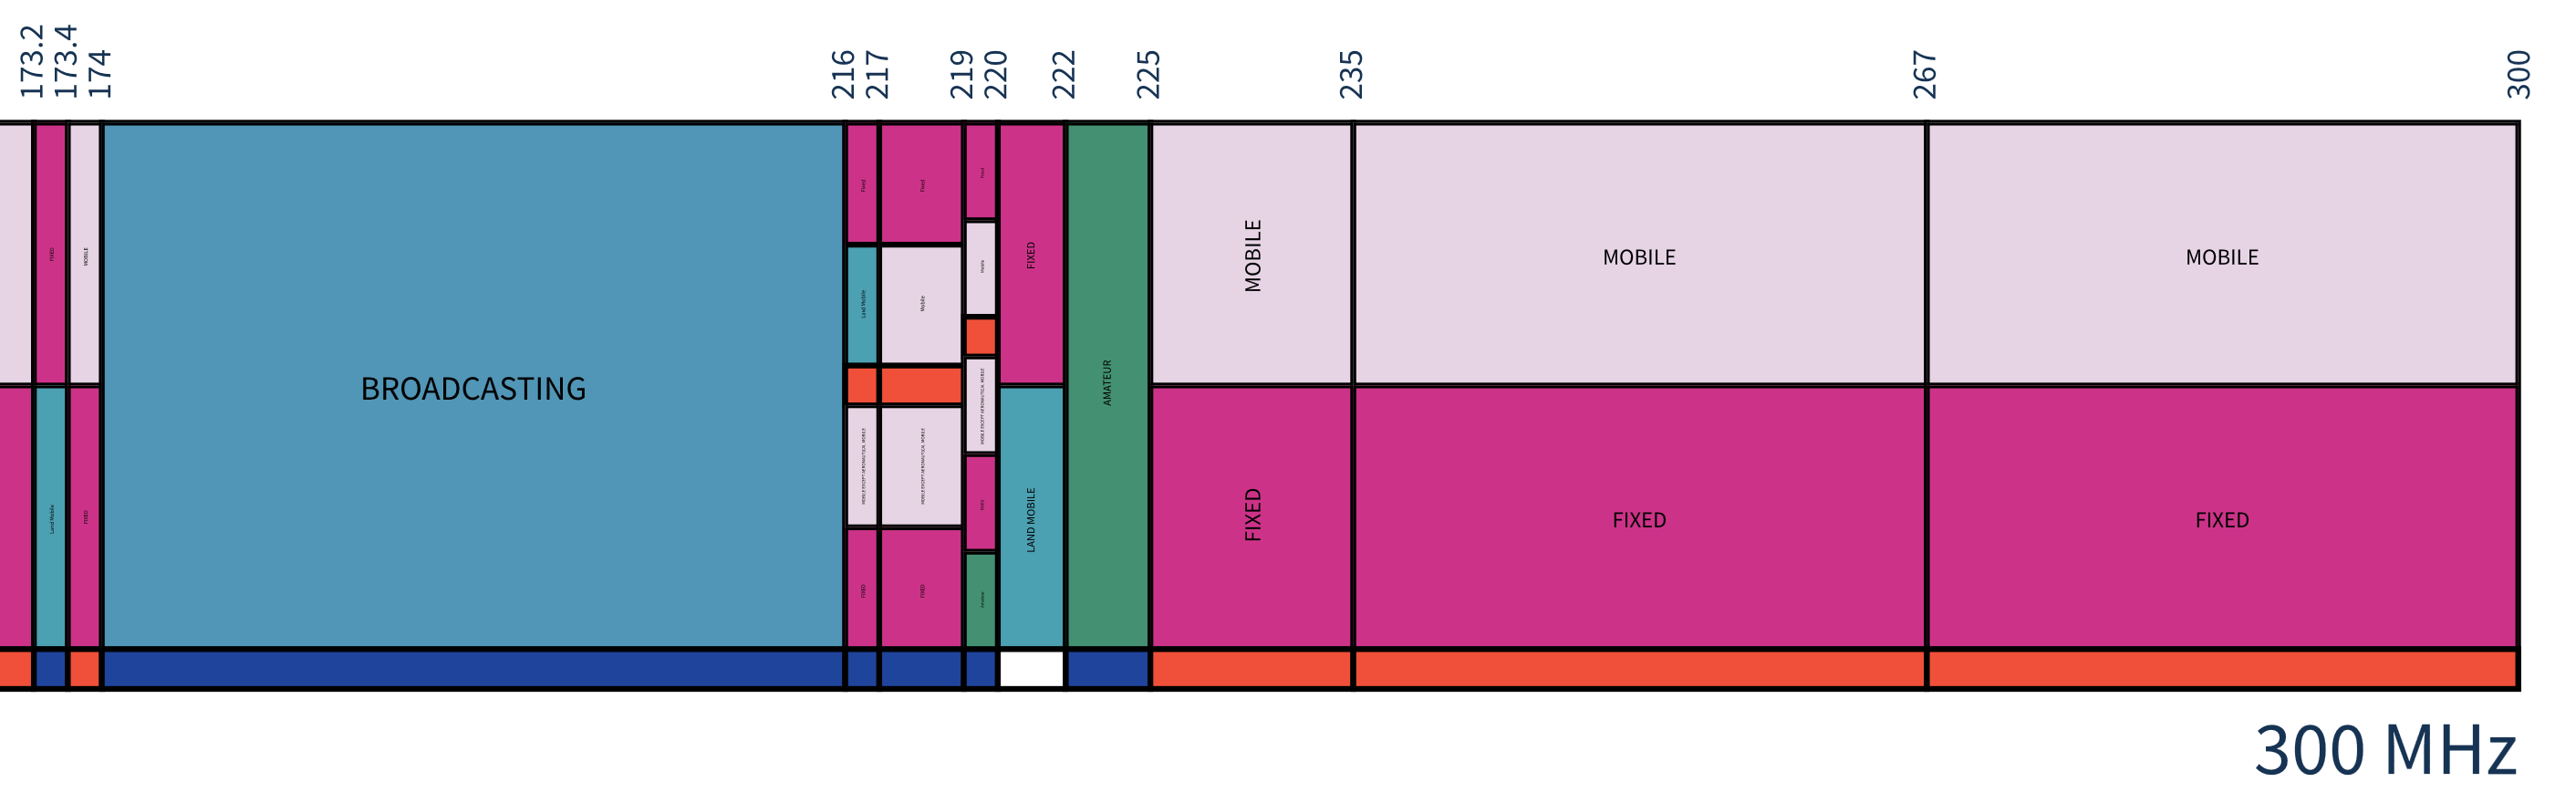
\includegraphics[width=0.9\linewidth]{images/section-1/radio-spectrum-usa-300.png}
    \caption{Radio Spectrum Allocation USA @\qty{300}{\mega\hertz}~\cite{radio-spectrum-usa}}
  \end{figure}
  \begin{itemize}
    \item Broadcasting starting @\qty{174}{\mega\hertz}: TV Channels
    \item Fixed/mobile starting @\qty{225}{\mega\hertz}: Military Band
      \begin{itemize}
        \item Primary military (e.g., air-to-air/air-to-ground voice)
        \item Aeronnautical radionavigation (instrument landing system (ILS) vertical guidance)
      \end{itemize}
  \end{itemize}
\end{frame}

\begin{frame}{Allocation Example II}
  \begin{columns}
    \begin{column}{0.56\textwidth}
      Frequency band \SIrange{2.4}{2.5}{\giga\hertz}
      \begin{itemize}
        \item Primary \ac{acro:ism} band
          \begin{itemize}
            \item High-power non-communication emitters (e.g., Microwave ovens, industrial heating and drying)
            \item Source of interference
          \end{itemize}
        \item Unlicensed wireless systems
          \begin{itemize}
            \item e.g., Wi-Fi, Bluetooth
            \item Must tolerate ISM interference
          \end{itemize}
      \end{itemize}
    \end{column}
    \begin{column}{0.38\textwidth}
      \begin{figure}
        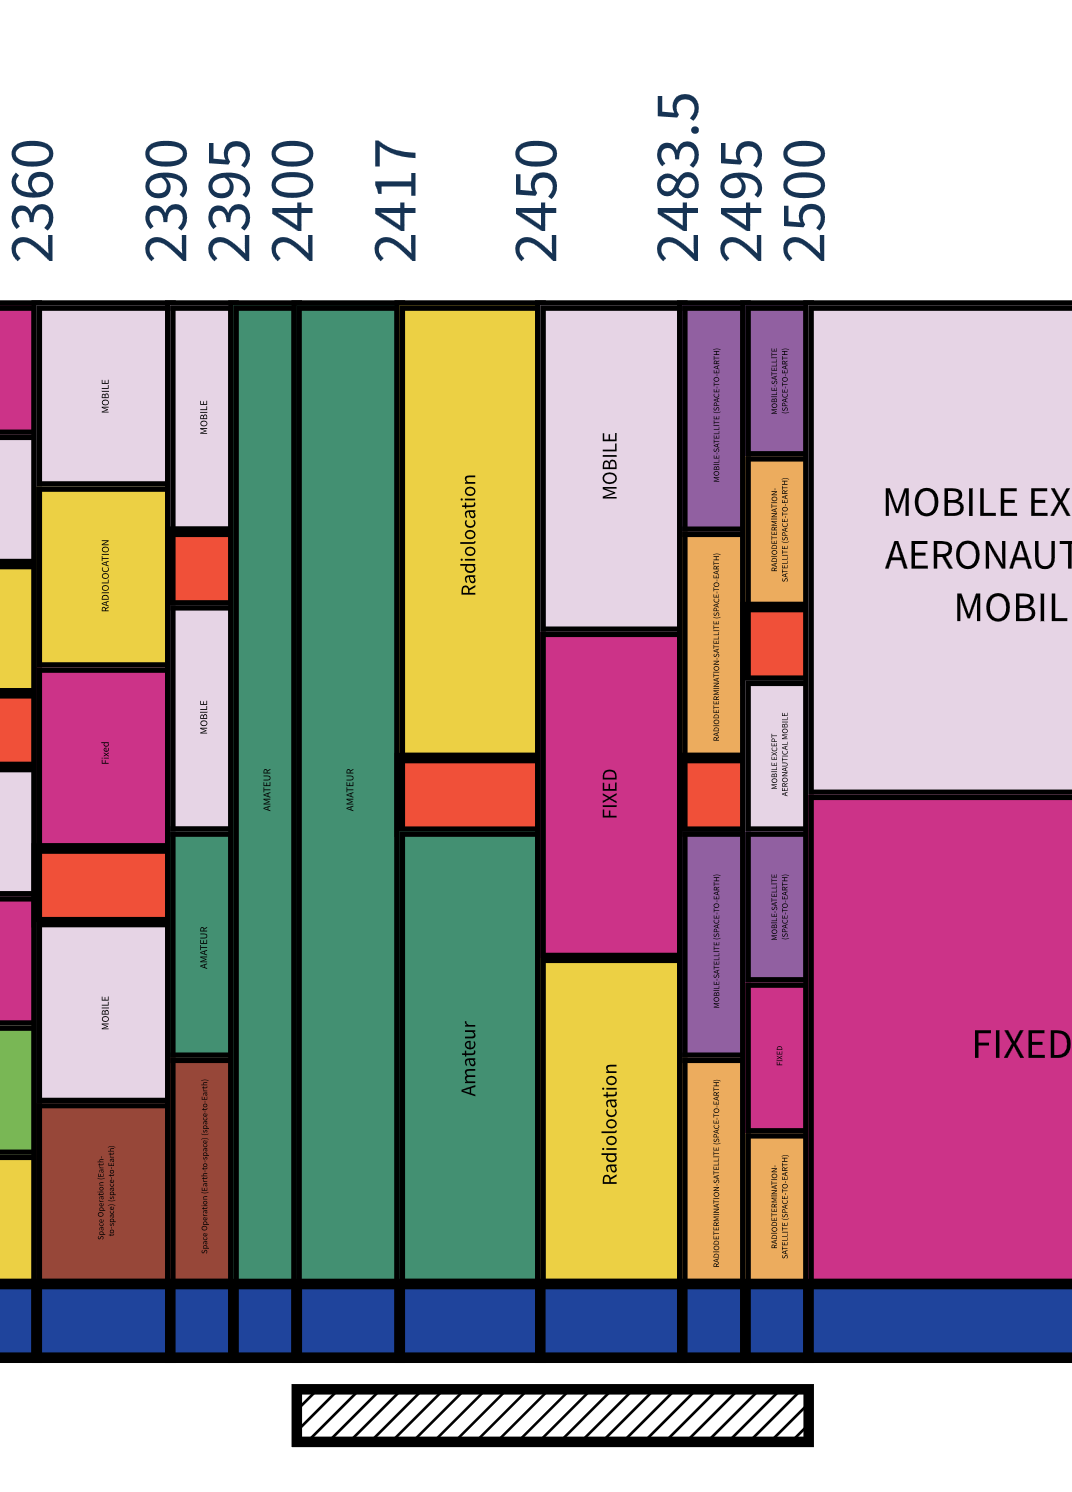
\includegraphics[width=0.6\linewidth]{images/section-1/radio-spectrum-usa-2400.png}
        \caption{Radio Spectrum Allocation USA @\qty{2.4}{\giga\hertz}~\cite{radio-spectrum-usa}}
      \end{figure}
    \end{column}
  \end{columns}
\end{frame}

\begin{frame}{ITU}
  \begin{columns}[T,onlytextwidth]
    \begin{column}{0.58\textwidth}
      \begin{itemize}
        \item United Nations Specialized Agency for Information and Communications Technology
        \item Founded in 1865 as the International Telegraph Union
        \item Renamed in 1947 to c{acro:itu}
        \item Coordinates global use of the radio spectrum
        \item In total 194 member states
        \item Each member state has equal representation and voting rights e.g., on standards
      \end{itemize}
    \end{column}
    \begin{column}{0.38\textwidth}
      \begin{block}{c{acro:itu}'s three sectors}
        \begin{itemize}
          \item c{acro:itu}-R (Radio): Radio spectrum management, satellite coordination
          \item c{acro:itu}-T (Telecommunication): Technical standards (Recommendations)
          \item c{acro:itu}-D (Development): Digital development in member states
        \end{itemize}
      \end{block}
    \end{column}
  \end{columns}
\end{frame}

\begin{frame}{Standards}
  \begin{columns}[onlytextwidth]
    \begin{column}{0.48\textwidth}
      \begin{itemize}
        \item Ensures fit for purpose, safe, and reliable products/services
        \item Promotes interoperability between equipment
        \item Harmonizes trade requirements across the globe
        \item Eliminates technical barriers
        \item \alert{Remark:} Standards are adopted by mutual consensus; some become legally binding through regulatory reference (e.g., \ac{acro:etsi} standards cited in \ac{acro:eu} law---USB-C in the \ac{acro:eu} common charger directive)
      \end{itemize}
    \end{column}
    %
    \begin{column}{0.5\textwidth}
      \begin{block}{What is a standard?}
        A standard is an agreed-upon, repeatable technical specification or guideline designed to ensure that materials, products, processes, and services are safe, reliable, and mutually interoperable.
      \end{block}
      \begin{block}{Key characteristics of radio standards}
        \begin{itemize}
          \item Consensus-based: agreed by all parties
          \item Documented: published and accessible
          \item Voluntary: adoption is typically optional
          \item Continuously updated: revised as technology evolves
        \end{itemize}
      \end{block}
    \end{column}
  \end{columns}
\end{frame}


\begin{frame}{Standardization Bodies I}
  Standardization bodies develop, approve, and publish standards.
  \begin{columns}[onlytextwidth]
    \begin{column}{0.6\textwidth}
      \begin{itemize}
        \item International bodies
          \begin{itemize}
            \item Coordinate global standards
            \item e.g., \ac{acro:iso} (from Greek \textit{isos}: equal)
            \item e.g., ITU
          \end{itemize}
        \item Regional bodies
          \begin{itemize}
            \item Cover large geographic areas
            \item e.g., \ac{acro:etsi}
          \end{itemize}
        \item National bodies
          \begin{itemize}
            \item Represent each country
            \item e.g., \ac{acro:din}
            \item e.g., \ac{acro:ansi}
          \end{itemize}
        \item Industry consortia
          \begin{itemize}
            \item Cover specific sectors
            \item e.g., \ac{acro:3gpp}
            \item e.g., \ac{acro:ieee}
          \end{itemize}
      \end{itemize}
    \end{column}
    \begin{column}{0.38\textwidth}
      \begin{block}{Role of industry consortia}
        \begin{itemize}
          \item Standards of big alliances are directly adopted into official frameworks\\
          \item Consortium defines specs $\rightarrow$ adopted as regional standard $\rightarrow$ recognized globally
          \item e.g., Cellular standard (5G \ac{acro:nr})
        \end{itemize}
        \centering
        \ac{acro:3gpp} (TS 38.211)\\
        $\downarrow$\\
        \ac{acro:etsi} (TS 138 211)\\
        $\downarrow$\\
        ITU-R (IMT-2020)\\
      \end{block}
    \end{column}
  \end{columns}
\end{frame}

\begin{frame}{Standardization Bodies II}
  \begin{columns}[T,onlytextwidth]
    \begin{column}{0.5\textwidth}
      IEEE
      \begin{itemize}
        \item Global professional association
        \item Develops technical standards for electronics and computing
        \item e.g., \ac{acro:ieee} 802.11 (Wi-Fi), 802.3 (Ethernet), 754 (floating-point)
      \end{itemize}
      ISO
      \begin{itemize}
        \item Network of national standards bodies
        \item Develops international standards across all industries
        \item e.g., \ac{acro:iso} 9001 (quality), \ac{acro:iso} 27001 (security), \ac{acro:iso}/\ac{acro:iec} 14443 (RFID/NFC)
      \end{itemize}
    \end{column}
    \begin{column}{0.5\textwidth}
      DIN
      \begin{itemize}
        \item German national standards body
        \item Representative for ISO/IEC
        \item \ac{acro:din} A4 paper, \ac{acro:din} 7258 (screws)
      \end{itemize}
      \vspace{2.5em}
      3GPP
      \begin{itemize}
        \item Collaboration of telecommunications standards organizations
        \item Develops specifications for mobile networks
        \item e.g., 3G, 4G, 5G, 6G
      \end{itemize}
    \end{column}
  \end{columns}
\end{frame}

\begin{frame}{Standardization Process I}
  \begin{columns}
    \begin{column}{0.48\textwidth}
      Types of standardization process
      \begin{itemize}
        \item Emergence as de facto standard (e.g., Ethernet)
        \item Written by standards organization (e.g., ITU-T Recommendations)
        \item Written by government or regulatory body (e.g., \ac{acro:fcc} rules)
        \item Written by a corporation (e.g., Apple Lightning connector)
      \end{itemize}
    \end{column}
    \begin{column}{0.5\textwidth}
      \begin{alertblock}{Standardize standards}
        The process of standardization can itself be standardized (e.g., \ac{acro:iso}/\ac{acro:iec} Directives Part 1/2).
        \begin{figure}
          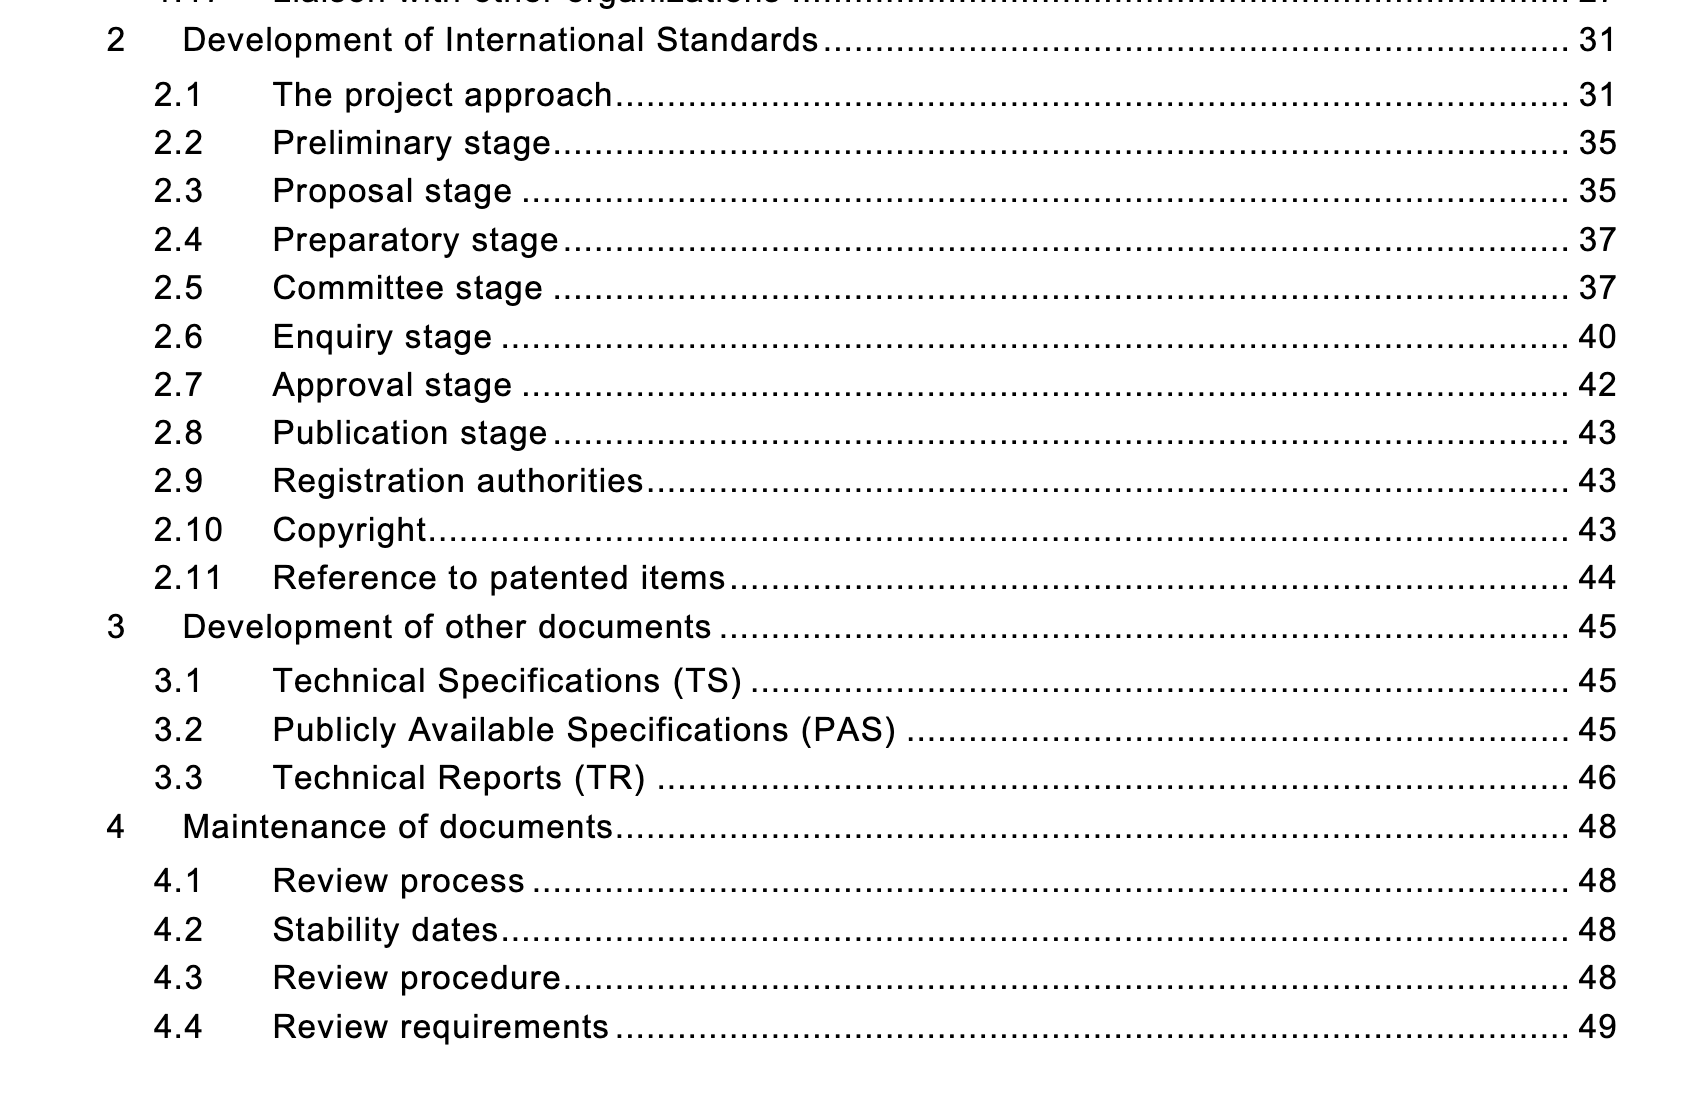
\includegraphics[width=0.8\linewidth]{images/section-1/iso-iec-overview.png}
          \caption{Excerpt from \ac{acro:iso}/\ac{acro:iec} Directives Part 1~\cite{iso-iec-overview}}
        \end{figure}
      \end{alertblock}
    \end{column}
  \end{columns}
\end{frame}

\begin{frame}{Standardization Process II}
  \begin{columns}[T,onlytextwidth]
    \begin{column}{0.58\textwidth}
      Standards are versioned through releases, e.g., 3GPP
      \begin{center}
        Release 8 (\ac{acro:lte})\\
        $\downarrow$\\
        Release 15 (5G)\\
        $\downarrow$\\
        Release 21 (6G)
      \end{center}
      \begin{itemize}
        \item Each release adds new features, fixes, and deprecations
        \item Industry coordinates on specific release versions
        \item Development can take years (especially for international bodies)
        \item Requires broad stakeholder participation
        \item Iterative process with multiple review rounds
      \end{itemize}
    \end{column}
    \begin{column}{0.38\textwidth}
      \begin{block}{Standardization Process (simplified)}
        \begin{enumerate}
          \item Propose new topic or revision
          \item Form working group of experts
          \item Draft, review, and refine the specification
          \item Achieve consensus and publish
          \item Maintain and periodically review
        \end{enumerate}
      \end{block}
    \end{column}
  \end{columns}
\end{frame}

\begin{frame}{Standardization Process III}
  \begin{figure}
    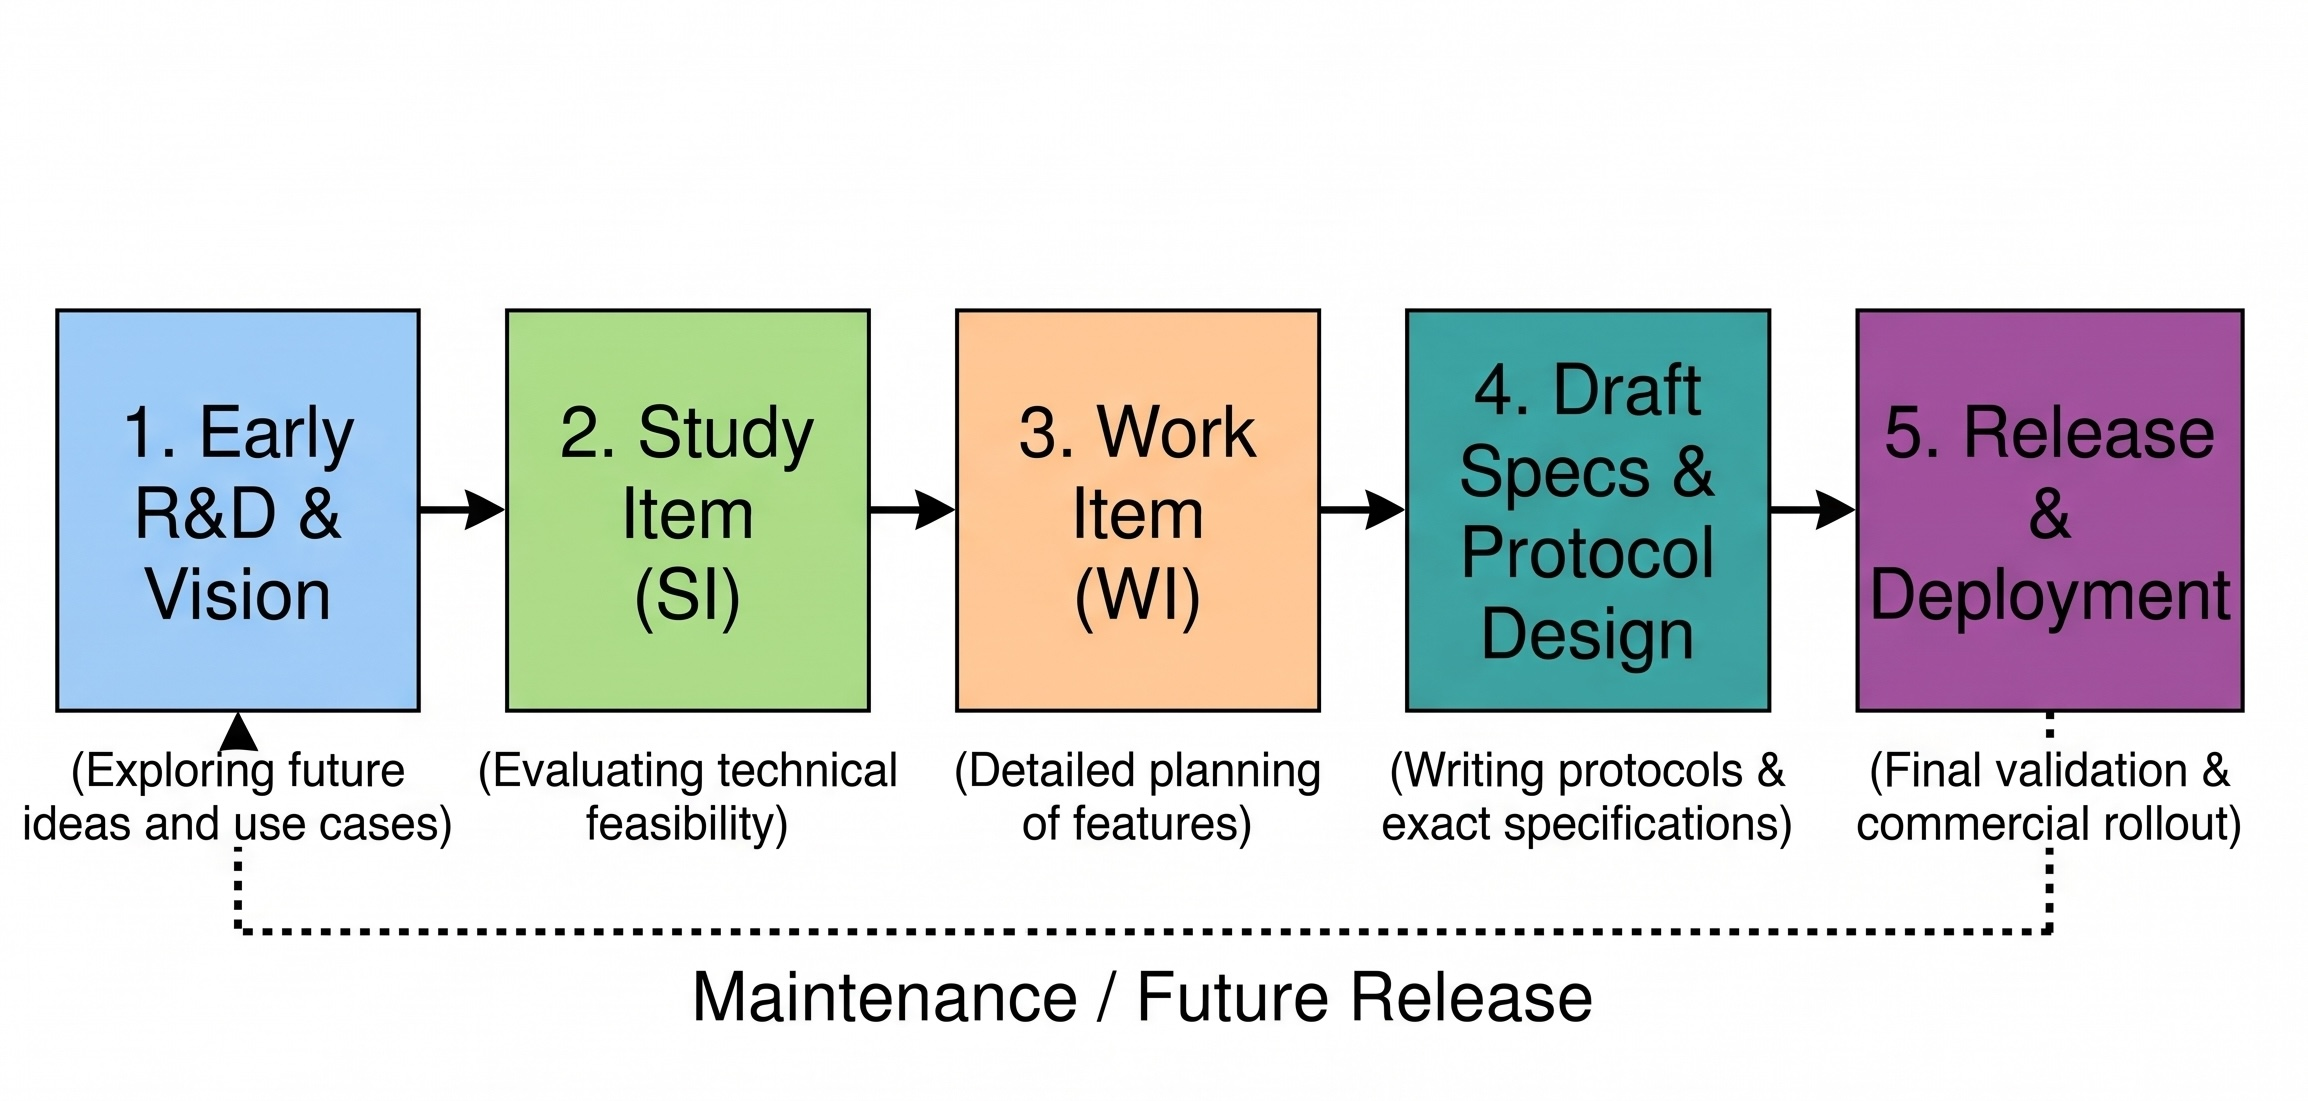
\includegraphics[width=1.0\linewidth]{images/section-1/3gpp-process.jpg}
    \caption{Standardization Process in 3GPP~\cite{gemini-imagen}}
  \end{figure}
\end{frame}

\begin{frame}{Standardization Process IV}
  \begin{figure}
    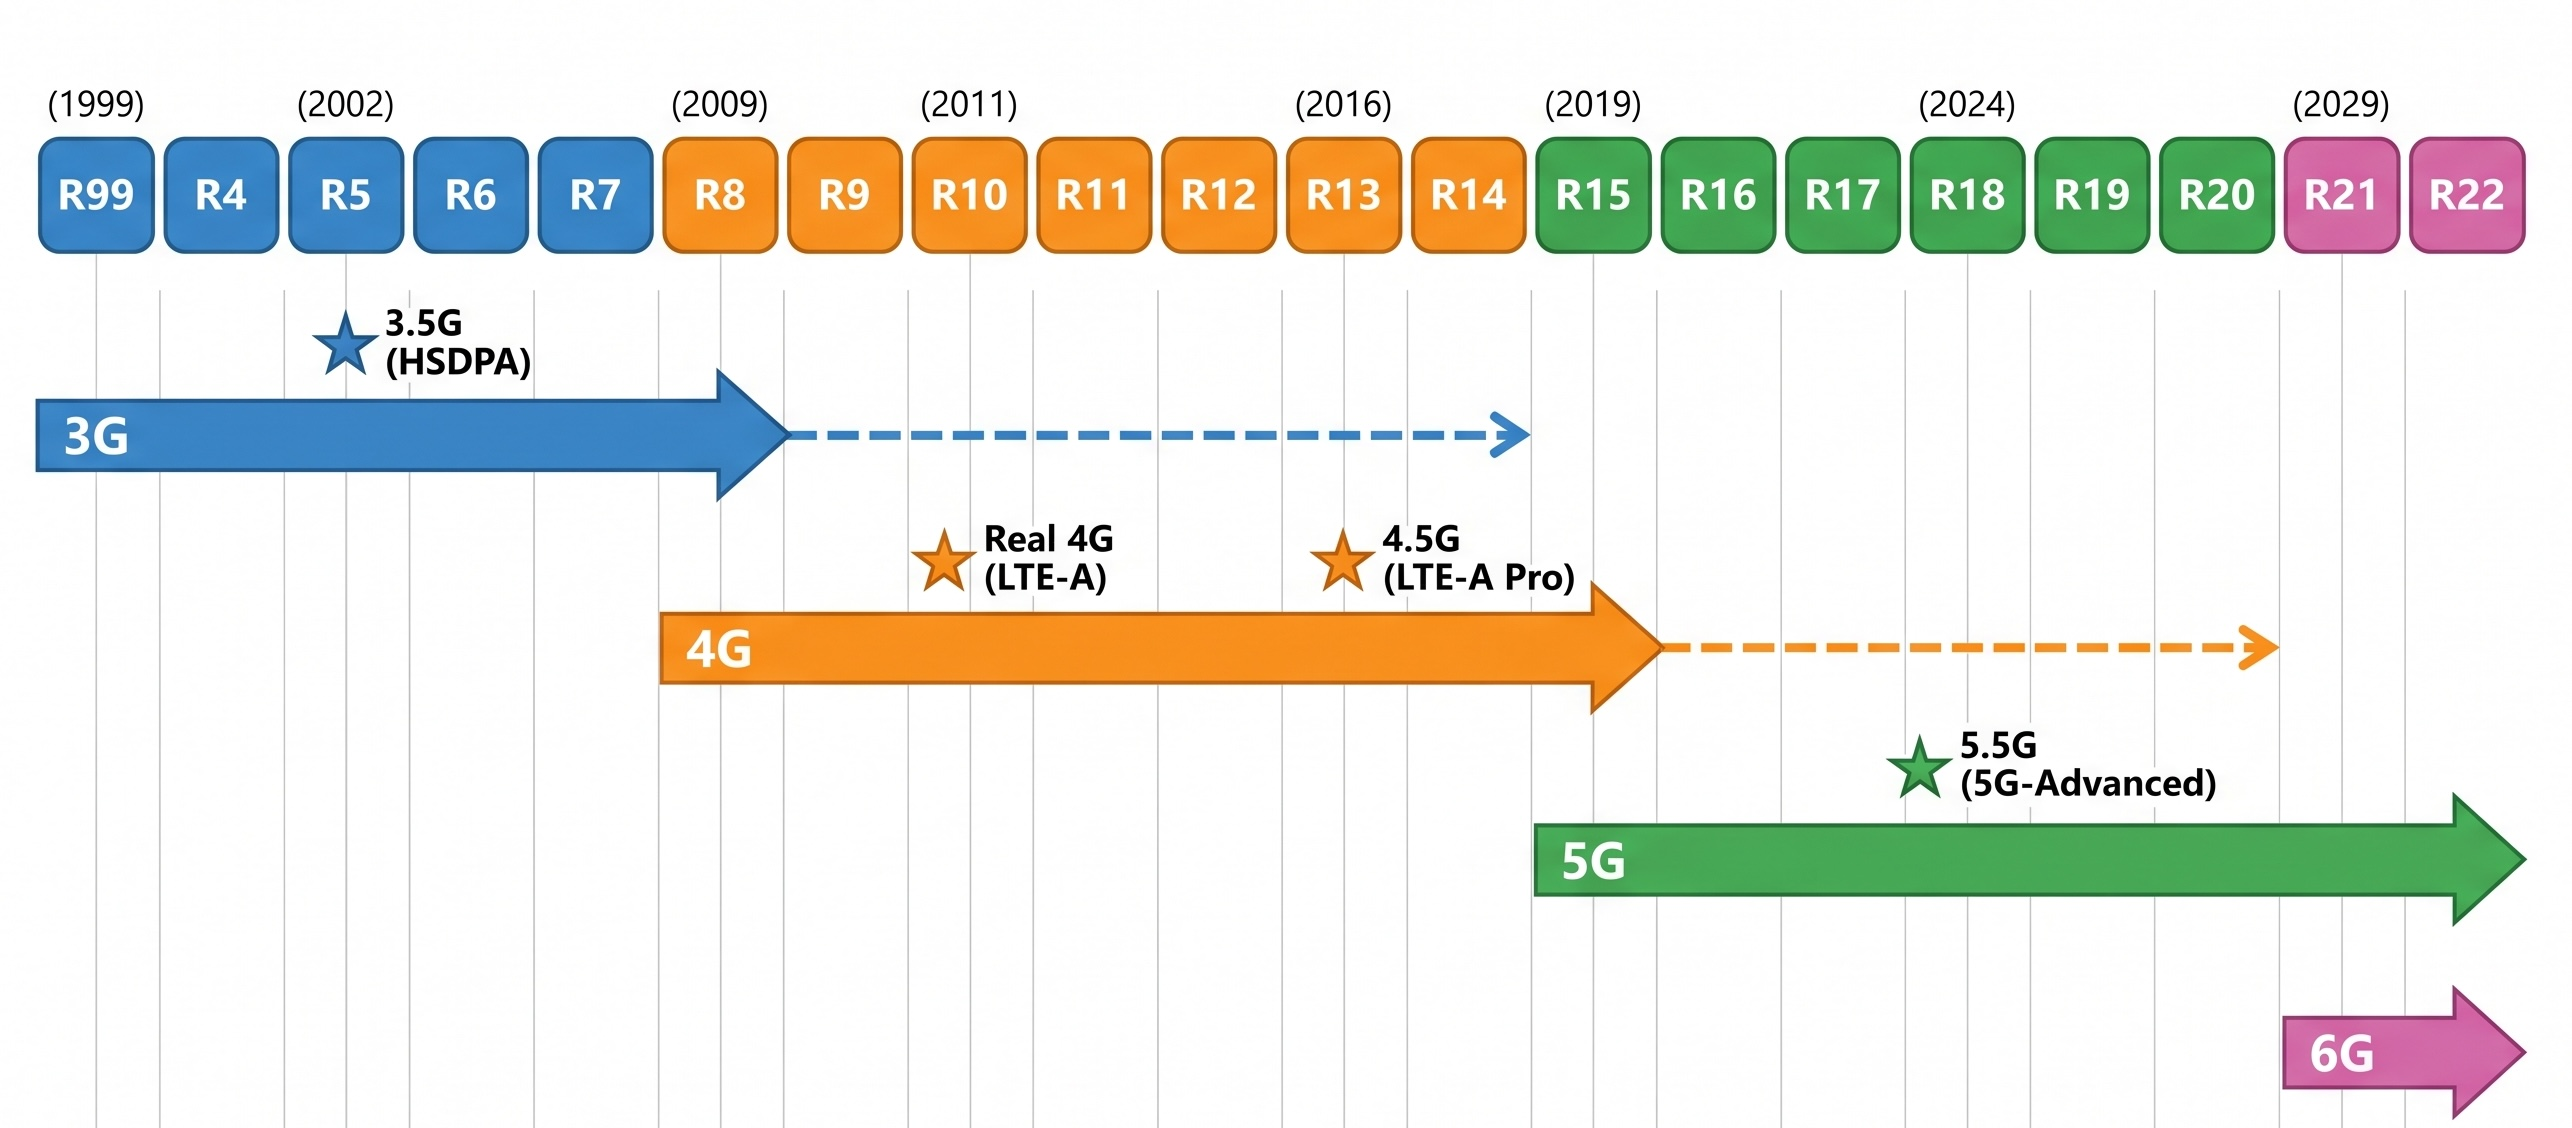
\includegraphics[width=0.8\linewidth]{images/section-1/3gpp-releases.jpg}
    \caption{Releases in \ac{acro:3gpp} over Time~\cite{gemini-imagen}}
  \end{figure}
\end{frame}

\begin{frame}{Patents I}
  Standards and patents intersect in radio systems, because standards often rely on patented innovations.
  \begin{columns}[onlytextwidth]
    \begin{column}{0.55\textwidth}
      \begin{itemize}
        \item Patent protects new technical solutions or  products
        \item Grants patent holder monopoly for up to 20 years
        \item Prohibits making, using, or selling the invention
        \item However, inventor publicly discloses the invention
      \end{itemize}
      Requirements for patentability
      \begin{itemize}
        \item Novelty: Invention must be new
        \item Inventive step: Invention not obvious to skilled person
        \item Industrial application: Invention can be made or used
      \end{itemize}
    \end{column}
    %
    \begin{column}{0.4\textwidth}
      \begin{block}{What is a patent?}
        A patent is an exclusive right granted for an invention.
      \end{block}
      \begin{block}{Patent process (simplified)}
        \begin{enumerate}
          \item File application with patent office
          \item Formal examination (completeness)
          \item Search for prior art
          \item Substantive examination (novelty, inventiveness, applicability)
          \item Grant or rejection
          \item Maintain with annual renewal fees
        \end{enumerate}
      \end{block}
    \end{column}
  \end{columns}
\end{frame}

\begin{frame}{Patents II}
  \begin{columns}[onlytextwidth]
    \begin{column}{0.6\textwidth}
      \ac{acro:sep}
      \begin{itemize}
        \item Patents that claim technology necessary to implement a standard
        \item e.g., \ac{acro:ofdm}A, channel coding, \ac{acro:mimo} schemes in 5G
        \item Any compliant device must use the patented technology
        \item Patent holder cannot exclude others from the standard market
      \end{itemize}
      \ac{acro:frand} commitment
      \begin{itemize}
        \item \textbf{F}air, \textbf{r}easonable, \textbf{a}nd \textbf{n}on-\textbf{d}iscriminatory
        \item \ac{acro:sep} holders commit to license on \ac{acro:frand} terms
        \item Balances innovation incentives with standard adoption
      \end{itemize}
    \end{column}
    \begin{column}{0.36\textwidth}
      \begin{block}{\ac{acro:frand} principle}
        \begin{itemize}
          \item Standardization increases patent value (must-use technology)
          \item \ac{acro:frand} limits royalty rates
          \item Tension between patent protection and open standards
        \end{itemize}
      \end{block}
    \end{column}
  \end{columns}
\end{frame}